\section{Method and Results}

\subsection{Task 1}

This task involved investigating the speed distribution of a gas of 
hard disks using event-driven simulation. A large number of particles 
were initialized with random positions and velocities. 
The initial speed distribution was a delta function. 
The system was left to reach equilibrium, and a new histogram 
of the speed distribution was created. The expected distribution 
was the 2D Maxwell-Boltzmann distribution, which was compared to 
the simulated result. It was decided that the simulation was going 
to try and simulate oxygen gas. 

To solve this task, 4 classes were made. Position, Velocity, 
Particle and System. Using a class structure means that the 
program has a large overhead but it also runs fast and is easy 
to understand. The class System, keeps track of all the particles 
in a list and all the collisions in a priority queue. System also 
has many memberfunctions, to calculate the systems energy, find all 
potensial collision and when they will occur, and basic return functions, 
which return the values we are interrested in and attributes such as 
elasticity, dt t\_c and more.

In order to compare the simulation to the boltsmann distribution, 
the mean\_velocity used in the simulation and the temperature used 
in the boltsmann function had to fullfill the equipartion theorem. 

\begin{equation}
E = N K_b T
\label{equipartion}
\end{equation}



Where the energy is the average energy of the gass for N 
number of particles at a temperatur of T. Since the energy of 
the gass is given by the kinetic energy of its gass particles. 
\autoref{equipartion} can be rewritten into the velocity of one 
particle as follows.

\begin{equation}
    v = \sqrt{\frac{2 k_b T}{m}}
\label{rms}
\end{equation}


The initial conditions used in the setup are 
given in the table below. The constant b refers to 
the volume taken up by one mole of $O_2$. The \autoref{Van} is a 
modified version of the ideal gass law. It is almost the same as 
the Ideal gass law, but with an extra term b to take into account 
that the gass particles are hard spheres.

The number of particles was set to 5000, elasticity was 1 and tc = 0. 

\begin{equation}
    V = n b + \frac{n R T }{P}
\label{Van}
\end{equation}

\autoref{Van} gives the volume of the gass, and is used 
to decide the dimensions of the box.


    


\begin{table}[h!]
\centering
\begin{tabular}{||c c ||} 
 \hline
    parameter & value  \\ 
  \hline\hline 
  $ k_b $& $1.38 \cdot 10^{-23}$ \\
  $R$ &$ 8.3144626$\\ 
  $b$ & $0.03186$  \cite{b}\\
  $v_{mean}$ & $461.3$ \\
  $T$ & $409.6 K$ \\
  $\mu$ & $1.66 \cdot 10^{-27}$\\
  $m_{O_{2}}$ & $32 \mu$ \\
  $P $& $101325 Pa$ \\
  $r_02$ & $152 \cdot 10{-12}$\\
  $mol$ &  $6.0221415 \cdot 10^{23}$\\
  $x = y$ &$ 8.161083 \cdot 10^{-8} $\\
 \hline
\end{tabular}
\end{table}


To check that the simulation had converged, the variance 
of the velocity distribution was calculated. As the system 
goes toward an equilibrium the change in variance will go 
towards zero. In other words the shape of the histogram
 will be constant.  


 \begin{figure}[ht]
    \centering
    \animategraphics[autoplay, loop, width = 0.1\textwidth]{12}{images/task1_n=2000/task1_n=2000-}{0}{69}
    \caption{task2 - mass 4m }
\end{figure}

\subsection{Task 2}
In this task, a gas mixture was simulated with 
two different types of particles having different 
masses. Half of the particles had a mass of m=m0, 
while the other half had a mass of m=4m0, where m0 was a 
constant. The goal was to plot the speed distribution 
histogram separately for both particle types before and 
after the system reached equilibrium. Additionally, 
the average speed and kinetic energy were calculated 
separately for each particle type. The value of the parameter 
eta used in this problem was 1.

The parameters were the same as in task 1. 

\begin{figure}[ht]
    \centering
    \animategraphics[autoplay, loop, width = 0.1\textwidth]{12}{images/task2_m_n/task2_m_n=2000-}{0}{69}
    \caption{task2 - mass m}
\end{figure}
 


\begin{figure}[ht]
    \centering
    \animategraphics[autoplay, loop, width = 0.1\textwidth]{12}{images/task2_4m_n/task2_4m_n=2000-}{0}{69}
    \caption{task2 - mass 4m }
\end{figure}


\begin{escapemulticol}
\begin{figure}[ht]
    \centering
    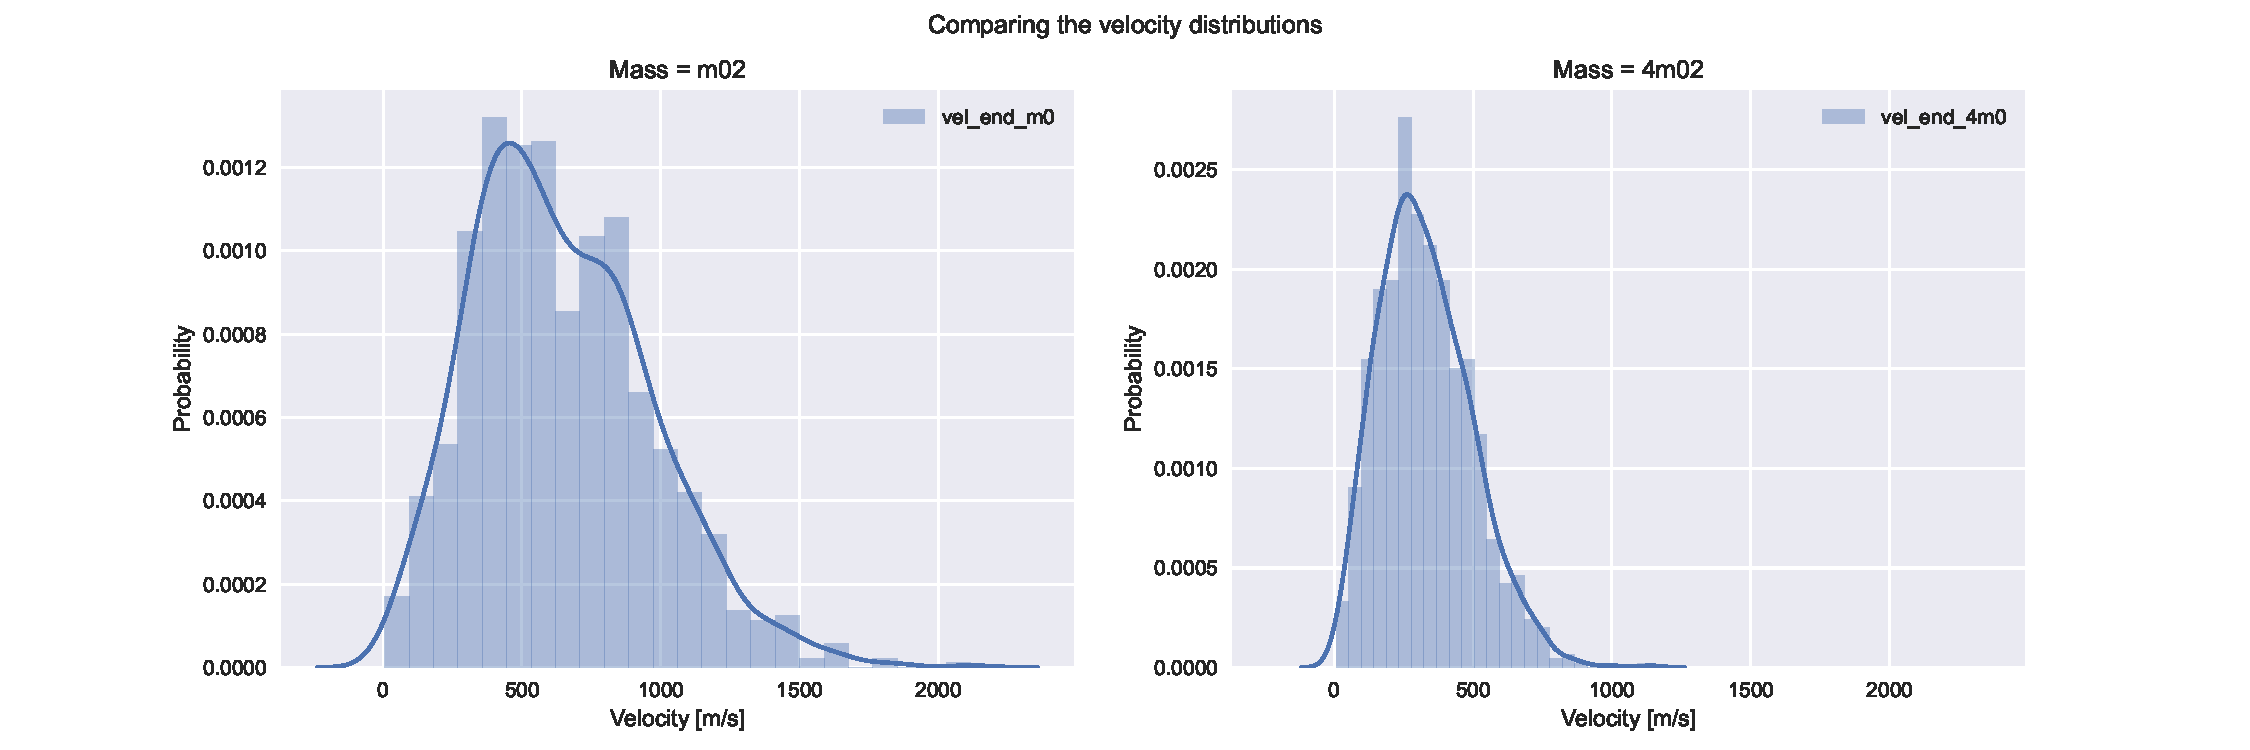
\includegraphics[width = \textwidth]{sections/images/Comparing_distributions_for_diff_mass.pdf}
    \caption{Figuren viser nøyaktighet, gitt tre ulike taps funksjoner. }
    \label{fig:task2_}
\end{figure}

\begin{figure}[ht]
    \centering
    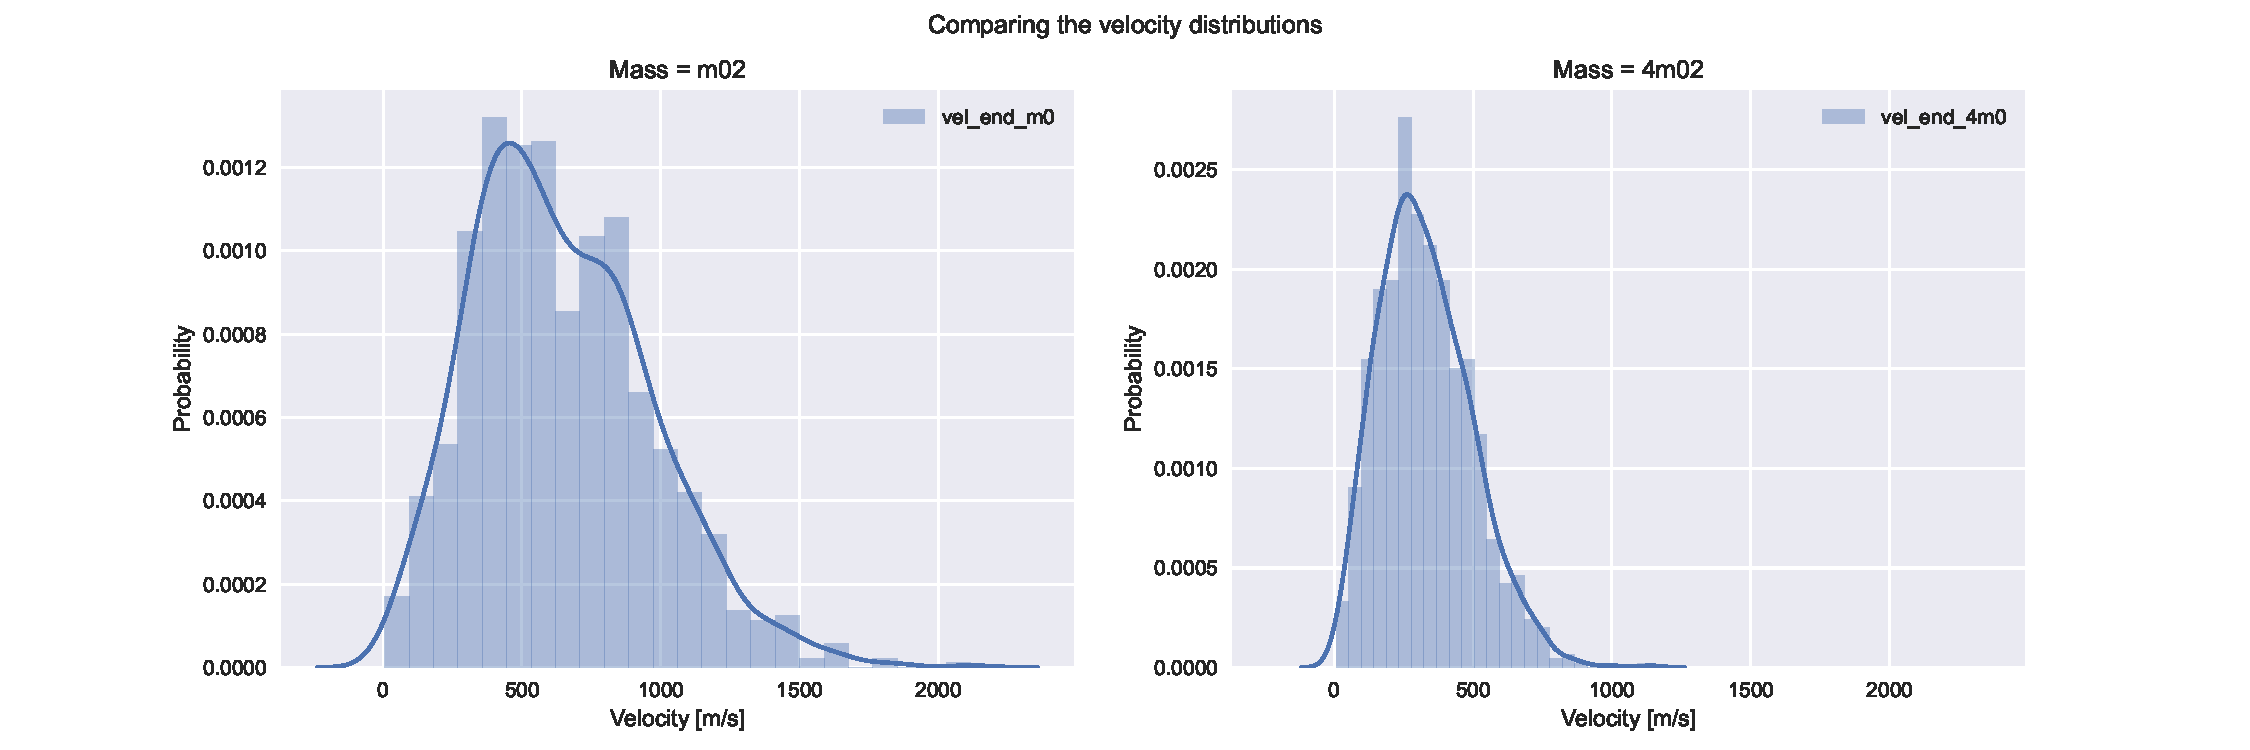
\includegraphics[width = \textwidth]{sections/images/Comparing_distributions_for_diff_mass.pdf}
    \caption{Figuren viser nøyaktighet, gitt tre ulike taps funksjoner. }
    \label{fig:loss}
\end{figure}

\begin{figure}[ht]
    \centering
    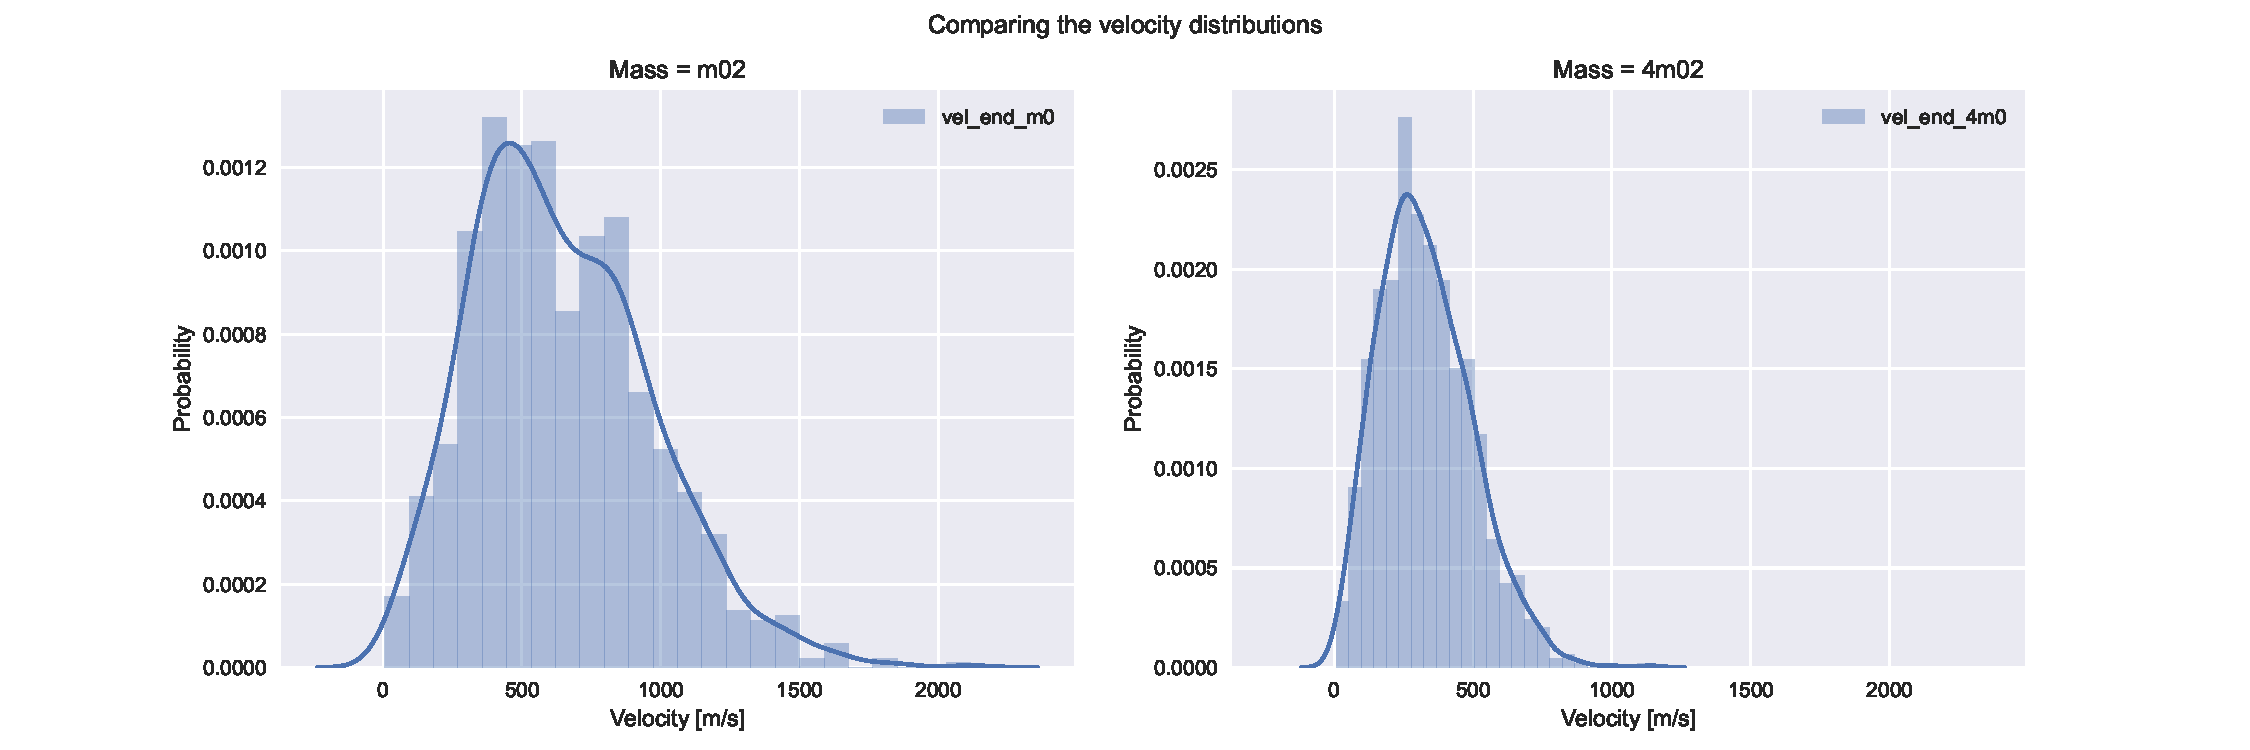
\includegraphics[width = \textwidth]{sections/images/Comparing_distributions_for_diff_mass.pdf}
    \caption{Figuren viser nøyaktighet, gitt tre ulike taps funksjoner. }
    \label{fig:loss}
\end{figure}

\end{escapemulticol}

\subsection{Task 3}

In this task, the objective was to repeat the setup of Problem 2 
and write output at short intervals, while ensuring that the 
average number of collisions per particle was much less than
 1 during an interval. At each output step, the average kinetic
  energy over all particles, the average over those particles with 
  mass m=m0, and the average over those with mass m=4m0 
  was calculated. The simulation was run until the average 
  number of particle-particle collisions per particle reached 10. 
  This procedure was repeated for eta=1, eta=0.9, and eta=0.8. 


